% Reading guide for Figs. 6 and 7 of juna_joint_ieee.tex (CL-221), in the
% format of the joint demodulation and decoding tutorial deck.  All wording
% from the two captions, equation (62), and the Experiment prose.
\documentclass[aspectratio=169,10pt]{beamer}
\usepackage[T1]{fontenc}
\usepackage{amsmath,amssymb,amsfonts}
\usepackage{bm}
\usepackage{tikz}
\usepackage{xcolor}
\usetikzlibrary{arrows.meta,positioning,shapes,calc}

\definecolor{parchment}{HTML}{F4E8C8}
\definecolor{paper}{HTML}{FAF1D8}
\definecolor{ink}{HTML}{1A1A1A}
\definecolor{inkgray}{HTML}{5A5A5A}
\definecolor{accentred}{HTML}{8B1A1A}
\definecolor{accentgreen}{HTML}{2D5F2C}
\definecolor{accentblue}{HTML}{1F4E79}
\definecolor{redbg}{HTML}{F7E0DE}
\definecolor{grnbg}{HTML}{E0EBDC}
\definecolor{blubg}{HTML}{DDE6EF}
\definecolor{labelbg}{HTML}{EFE0B0}

\usefonttheme{serif}
\setbeamercolor{background canvas}{bg=parchment}
\setbeamercolor{normal text}{fg=ink}
\setbeamercolor{structure}{fg=ink}
\setbeamercolor{frametitle}{fg=ink,bg=parchment}
\setbeamercolor{title}{fg=ink}
\setbeamercolor{itemize item}{fg=ink}
\setbeamercolor{itemize subitem}{fg=ink}
\setbeamercolor{item}{fg=ink}
\setbeamercolor{caption name}{fg=ink}
\setbeamertemplate{navigation symbols}{}
\setbeamertemplate{itemize item}{\textbullet}

\setbeamertemplate{frametitle}{%
  \vspace{0.30em}%
  \begin{center}%
    {\bfseries\Large\insertframetitle\par}%
    \vspace{0.28em}%
    {\color{ink}\rule{0.86\paperwidth}{0.4pt}}%
  \end{center}%
  \vspace{0.10em}%
}
\setbeamertemplate{footline}{%
  \hbox to \paperwidth{\hfil\itshape\small\insertframenumber\hspace{0.7em}}%
  \vspace{0.35em}%
}

\newcommand{\vY}{\bm{Y}}
\newcommand{\vy}{\bm{y}}
\newcommand{\vA}{\bm{A}}
\newcommand{\vB}{\bm{B}}
\newcommand{\valpha}{\bm{\alpha}}
\newcommand{\vn}{\bm{n}}
\newcommand{\vs}{\bm{s}}
\newcommand{\vW}{\bm{W}}
\newcommand{\T}{^{\mathsf T}}
\newcommand{\Hh}{^{\mathsf H}}
\newcommand{\norm}[1]{\left\lVert #1\right\rVert}
\DeclareMathOperator*{\argmin}{arg\,min}

\tikzset{
  flowbox/.style={draw=ink,fill=paper,line width=0.6pt,
                  minimum width=2.5cm,minimum height=1.0cm,
                  align=center,font=\small\bfseries,inner sep=4pt},
  smallbox/.style={draw=ink,fill=paper,line width=0.4pt,
                   minimum width=0.7cm,minimum height=0.55cm,
                   inner sep=2pt,align=center,font=\footnotesize\itshape},
  method/.style={draw=accentgreen,fill=grnbg,line width=1.0pt,
                 align=center,font=\small\bfseries,inner sep=6pt},
  issue/.style={draw=accentred,fill=redbg,line width=1.0pt,
                align=center,font=\small\bfseries,inner sep=6pt},
  idea/.style={draw=accentblue,fill=blubg,line width=1.0pt,
               align=center,font=\small\bfseries,inner sep=6pt},
  flowarr/.style={-{Stealth[length=2.5mm,width=2mm]},line width=0.7pt},
  softarr/.style={-{Stealth[length=2mm,width=1.6mm]},line width=0.5pt,color=inkgray}
}

\newcommand{\bottomnote}[1]{%
  \begin{center}{\itshape\small #1}\end{center}}

\newcommand{\papercover}[4]{%
  \begin{frame}[plain]
    \vfill
    \begin{center}
      {\bfseries\Huge #1\par}
      \vspace{0.8cm}
      {\Large #2\par}
      \vspace{0.35cm}
      {\itshape\large\color{inkgray}#3\par}
      \vspace{0.55cm}
      {\small\texttt{\detokenize{#4}}\par}
    \end{center}
    \vfill
  \end{frame}}

\newcommand{\twocolmodel}[4]{%
  \begin{columns}[T,onlytextwidth]
    \begin{column}{0.48\textwidth}#1\end{column}
    \begin{column}{0.48\textwidth}#2\end{column}
  \end{columns}
  \bottomnote{#3\\#4}}


\usetikzlibrary{fit,decorations.pathreplacing}
\graphicspath{{../../../juna_joint_ieee/figures/}}

\tikzset{
  card/.style={draw=ink,fill=paper,line width=0.55pt,rounded corners=2pt,
               align=center,inner sep=5pt,font=\small},
  goodcard/.style={draw=accentgreen,fill=grnbg,line width=0.85pt,
                   rounded corners=2pt,align=center,inner sep=5pt,font=\small},
  badcard/.style={draw=accentred,fill=redbg,line width=0.85pt,
                  rounded corners=2pt,align=center,inner sep=5pt,font=\small},
  bluecard/.style={draw=accentblue,fill=blubg,line width=0.85pt,
                   rounded corners=2pt,align=center,inner sep=5pt,font=\small},
  panelbox/.style={draw=ink,fill=parchment,line width=0.7pt,rounded corners=2pt},
  bluearr/.style={-{Stealth[length=2.5mm,width=2mm]},line width=0.85pt,
                   draw=accentblue},
  redarr/.style={-{Stealth[length=2.5mm,width=2mm]},line width=0.85pt,
                  draw=accentred}
}

\begin{document}

% =====================================================================
% 1. Cover
% =====================================================================
\begin{frame}[plain]
  \centering
  \vspace{0.30cm}
  {\small\color{inkgray}Figures 5--11 of \texttt{juna\_joint\_ieee.tex}\par}
  \vspace{0.22cm}
  {\bfseries\Huge Reading the Red Result Figures\par}
  \vspace{0.28cm}
  {\Large The measured channels, the payload bit error rate curves, the
   best observed rate, and the two maps that explain every point\par}
  \vspace{0.55cm}
  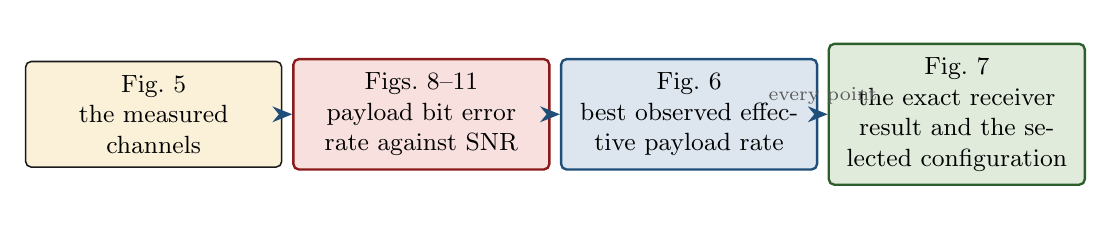
\begin{tikzpicture}[x=1cm,y=1cm]
    \path[use as bounding box] (-6.7,-1.3) rectangle (6.7,1.1);
    \node[card,text width=2.9cm] (f5) at (-5.1,0) {Fig.~5\\the measured
      channels};
    \node[badcard,text width=2.9cm] (f8) at (-1.7,0) {Figs.~8--11\\payload
      bit error rate against SNR};
    \node[bluecard,text width=2.9cm] (f6) at (1.7,0) {Fig.~6\\best observed
      effective payload rate};
    \node[goodcard,text width=2.9cm] (f7) at (5.1,0) {Fig.~7\\the exact
      receiver result and the selected configuration};
    \draw[bluearr] (f5) -- (f8);
    \draw[bluearr] (f8) -- (f6);
    \draw[bluearr] (f6) -- (f7)
      node[midway,above,font=\scriptsize,color=inkgray] {every point};
  \end{tikzpicture}
\end{frame}
% =====================================================================
% 1b. The measured channels
% =====================================================================
\begin{frame}{The measured channels}
  \centering
  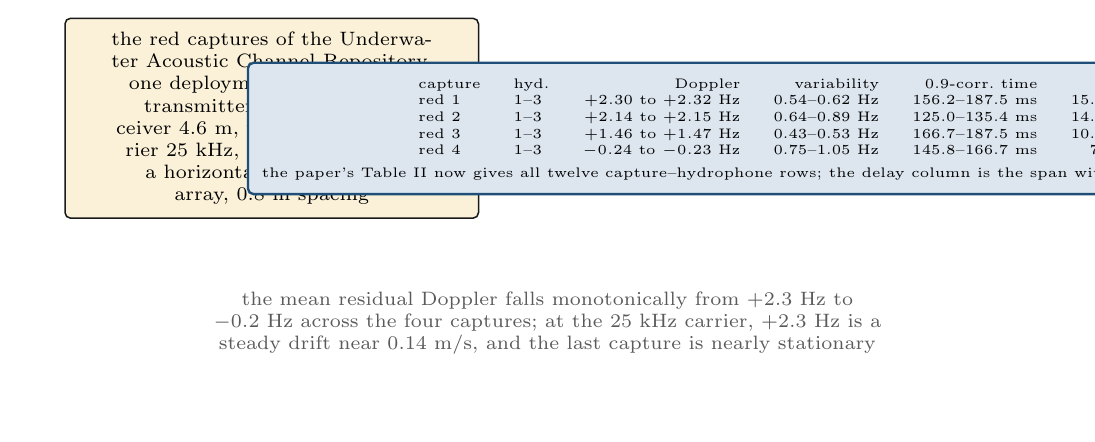
\begin{tikzpicture}[x=1cm,y=1cm]
    \path[use as bounding box] (-6.6,-2.9) rectangle (6.6,2.0);
    \node[card,text width=4.9cm,font=\scriptsize] at (-3.5,0.85)
      {the red captures of the Underwater Acoustic Channel Repository, one
       deployment in Singapore:\\transmitter depth 6~m, receiver 4.6~m,
       water 8--15~m, carrier 25~kHz, range 0.1--0.4~km;\\a horizontal
       three-element array, 0.8~m spacing};
    \node[bluecard,font=\tiny] at (3.3,0.72)
      {\begin{tabular}{@{}llrrrr@{}}
        capture & hyd. & Doppler & variability & 0.9-corr.\ time & 30~dB delay\\
        red 1 & 1--3 & $+2.30$ to $+2.32$~Hz & 0.54--0.62~Hz & 156.2--187.5~ms & 15.68--32.76~ms\\
        red 2 & 1--3 & $+2.14$ to $+2.15$~Hz & 0.64--0.89~Hz & 125.0--135.4~ms & 14.95--38.85~ms\\
        red 3 & 1--3 & $+1.46$ to $+1.47$~Hz & 0.43--0.53~Hz & 166.7--187.5~ms & 10.10--38.02~ms\\
        red 4 & 1--3 & $-0.24$ to $-0.23$~Hz & 0.75--1.05~Hz & 145.8--166.7~ms & 7.66--9.79~ms\\
       \end{tabular}\\[2pt]
       \tiny the paper's Table II now gives all twelve
       capture--hydrophone rows; the delay column is the span within
       30~dB of the strongest tap};
    \node[font=\scriptsize,color=inkgray,text width=11.6cm,align=center]
      at (0,-1.75)
      {the mean residual Doppler falls monotonically from $+2.3$~Hz to
       $-0.2$~Hz across the four captures; at the 25~kHz carrier,
       $+2.3$~Hz is a steady drift near 0.14~m/s, and the last capture is
       nearly stationary};
  \end{tikzpicture}
  \bottomnote{Four captures share this deployment record and differ only in
    their codenames; their measured statistics separate them.  Red 2 is the
    fastest path --- watch its row when the bit error rate figures arrive.}
\end{frame}

% ---------------------------------------------------------------------
\begin{frame}[plain]
  \centering
  \begin{tikzpicture}
    \node[anchor=south west,inner sep=0] (img) at (0,0)
      {\includegraphics[width=0.98\paperwidth,height=0.86\textheight,
        keepaspectratio]{red_channel_impulse_response}};
    \begin{scope}[x={(img.south east)},y={(img.north west)}]
      \only<2->{
      \node[draw=accentred,fill=paper,fill opacity=0.93,text opacity=1,line width=0.6pt,rounded corners=1.5pt,align=center,inner sep=2.5pt,font=\tiny,text width=2.8cm] (c5a) at (-0.60,0.88) {red 1: 30~dB spans 15.68--32.76~ms; late arrivals reach about 10~ms};
      \draw[redarr] (c5a.east) -- (0.02,0.88);
      \node[draw=accentred,fill=paper,fill opacity=0.93,text opacity=1,line width=0.6pt,rounded corners=1.5pt,align=center,inner sep=2.5pt,font=\tiny,text width=2.8cm] (c5g) at (-0.60,0.60) {the arrival structure rearranges between captures: consecutive-capture profile correlation 0.25--0.76};
      \draw[redarr] (c5g.east) -- (0.02,0.51);
      \node[draw=accentred,fill=paper,fill opacity=0.93,text opacity=1,line width=0.6pt,rounded corners=1.5pt,align=center,inner sep=2.5pt,font=\tiny,text width=2.8cm] (c5d) at (-0.60,0.34) {red 3: $+1.5$~Hz with the steadiest variability, 0.43--0.53~Hz};
      \draw[redarr] (c5d.east) -- (0.02,0.39);
      \node[draw=accentred,fill=paper,fill opacity=0.93,text opacity=1,line width=0.6pt,rounded corners=1.5pt,align=center,inner sep=2.5pt,font=\tiny,text width=2.8cm] (c5f) at (-0.60,0.10) {each box: the path's 30~dB delay span and its mean residual Doppler};
      \draw[redarr] (c5f.east) -- (0.28,0.045);
      \node[draw=accentred,fill=paper,fill opacity=0.93,text opacity=1,line width=0.6pt,rounded corners=1.5pt,align=center,inner sep=2.5pt,font=\tiny,text width=2.8cm] (c5b) at (1.60,0.88) {late arrivals thin from hydrophone~1 (left) to hydrophone~3 (right) in every row};
      \draw[redarr] (c5b.west) -- (0.98,0.88);
      \node[draw=accentred,fill=paper,fill opacity=0.93,text opacity=1,line width=0.6pt,rounded corners=1.5pt,align=center,inner sep=2.5pt,font=\tiny,text width=2.8cm] (c5c) at (1.60,0.58) {red 2: the fastest path --- 0.9-correlation time 125.0--135.4~ms, narrowly above the 106.7~ms useful interval for $N=1024$; the worst 30~dB span, 38.85~ms, on hydrophone~1};
      \draw[redarr] (c5c.west) -- (0.98,0.64);
      \node[draw=accentred,fill=paper,fill opacity=0.93,text opacity=1,line width=0.6pt,rounded corners=1.5pt,align=center,inner sep=2.5pt,font=\tiny,text width=2.8cm] (c5e) at (1.60,0.16) {red 4: nearly stationary, $-0.2$~Hz, the least multipath (7.66--9.79~ms), the most Doppler variation (0.75--1.05~Hz)};
      \draw[redarr] (c5e.west) -- (0.98,0.14);
      }
    \end{scope}
  \end{tikzpicture}\par
  {\tiny\color{inkgray}Fig.~5 of \texttt{juna\_joint\_ieee.tex}\par}
\end{frame}
% =====================================================================
% 8b. From capture to point
% =====================================================================
\begin{frame}{From capture to point}
  \centering
  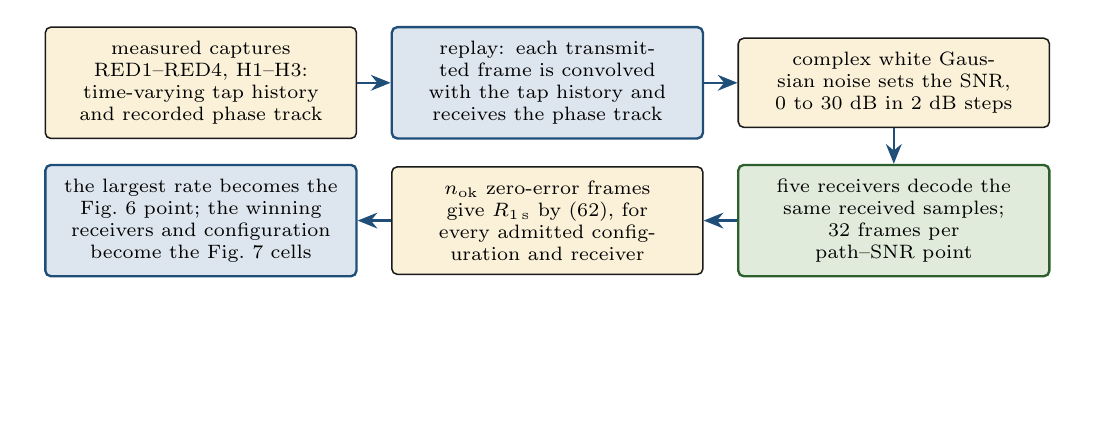
\begin{tikzpicture}[x=1cm,y=1cm]
    \path[use as bounding box] (-6.6,-2.9) rectangle (6.6,2.0);
    \node[card,text width=3.6cm,font=\scriptsize] (cap) at (-4.4,1.30)
      {measured captures\\RED1--RED4, H1--H3:\\time-varying tap history\\
       and recorded phase track};
    \node[bluecard,text width=3.6cm,font=\scriptsize] (rep) at (0,1.30)
      {replay: each transmitted frame is convolved with the tap history
       and receives the phase track};
    \node[card,text width=3.6cm,font=\scriptsize] (noise) at (4.4,1.30)
      {complex white Gaussian noise sets the SNR,\\0 to 30~dB in 2~dB
       steps};
    \node[goodcard,text width=3.6cm,font=\scriptsize] (dec) at (4.4,-0.45)
      {five receivers decode the same received samples;\\32 frames per
       path--SNR point};
    \node[card,text width=3.6cm,font=\scriptsize] (rate) at (0,-0.45)
      {$n_{\mathrm{ok}}$ zero-error frames give $R_{\mathrm{1\,s}}$
       by (62), for every admitted configuration and receiver};
    \node[bluecard,text width=3.6cm,font=\scriptsize] (fig) at (-4.4,-0.45)
      {the largest rate becomes the Fig.~6 point; the winning receivers
       and configuration become the Fig.~7 cells};
    \draw[bluearr] (cap) -- (rep);
    \draw[bluearr] (rep) -- (noise);
    \draw[bluearr] (noise) -- (dec);
    \draw[bluearr] (dec) -- (rate);
    \draw[bluearr] (rate) -- (fig);
  \end{tikzpicture}
  \bottomnote{Five receivers decode the same received samples at every
    point, so each comparison holds the frames, the channel, and the noise
    fixed.  Eighteen admitted configurations compete at every path--SNR
    point.}
\end{frame}

% =====================================================================
% 3. The grid
% =====================================================================
\begin{frame}{The grid}
  \centering
  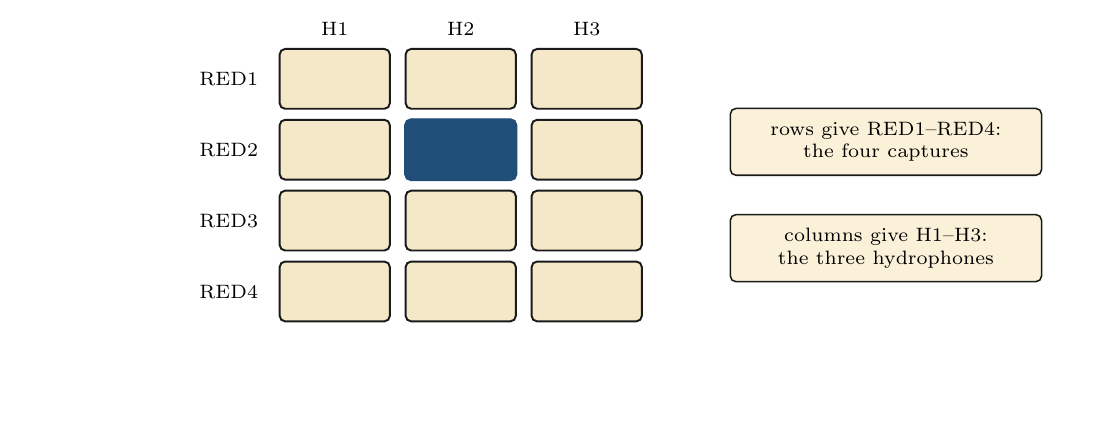
\begin{tikzpicture}[x=1cm,y=1cm]
    \path[use as bounding box] (-6.6,-2.9) rectangle (6.6,2.0);
    \foreach \r/\yy in {1/1.35, 2/0.45, 3/-0.45, 4/-1.35}{
      \node[font=\scriptsize,anchor=east] at (-3.55,\yy) {RED\r};
      \foreach \c/\xx in {1/-2.7, 2/-1.1, 3/0.5}{
        \draw[panelbox] (\xx-0.7,\yy-0.38) rectangle (\xx+0.7,\yy+0.38);
      }
    }
    \foreach \c/\xx in {1/-2.7, 2/-1.1, 3/0.5}{
      \node[font=\scriptsize,anchor=south] at (\xx,1.78) {H\c};
    }
    \draw[panelbox,line width=1.1pt,color=accentblue]
      (-1.8,0.07) rectangle (-0.4,0.83);
    \node[card,text width=3.6cm,font=\scriptsize] at (4.3,0.55)
      {rows give RED1--RED4:\\the four captures};
    \node[card,text width=3.6cm,font=\scriptsize] at (4.3,-0.80)
      {columns give H1--H3:\\the three hydrophones};
  \end{tikzpicture}
  \bottomnote{Twelve panels, one per capture--hydrophone path.  Each panel
    is read the same way; the marked panel is RED2 on H2.}
\end{frame}

% =====================================================================
% 8c. The payload bit error rate figures
% =====================================================================
\begin{frame}{The payload bit error rate figures}
  \centering
  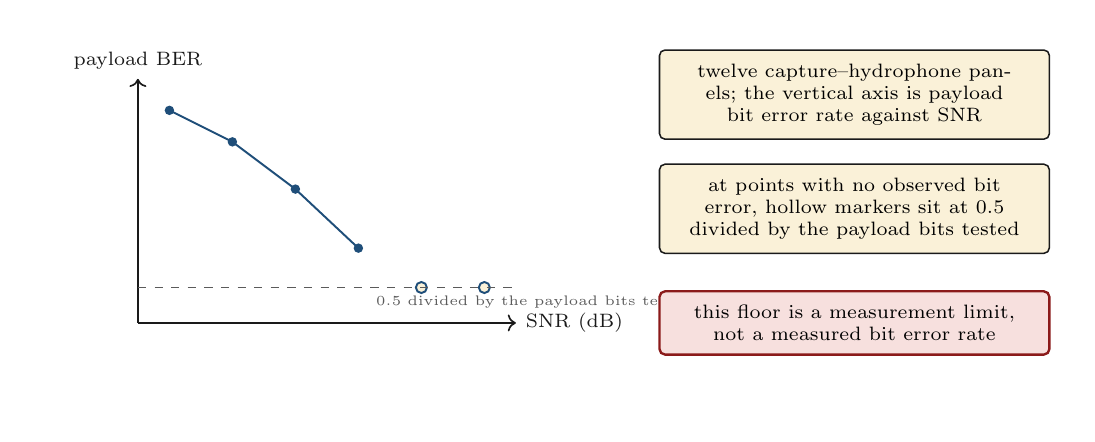
\begin{tikzpicture}[x=1cm,y=1cm]
    \path[use as bounding box] (-6.6,-2.9) rectangle (6.6,2.0);
    \begin{scope}[shift={(-2.9,-0.35)}]
      \draw[->,line width=0.6pt,color=ink] (-2.3,-1.4) -- (2.5,-1.4)
        node[right,font=\scriptsize] {SNR (dB)};
      \draw[->,line width=0.6pt,color=ink] (-2.3,-1.4) -- (-2.3,1.7)
        node[above,font=\scriptsize] {payload BER};
      \draw[line width=0.7pt,color=accentblue]
        (-1.9,1.30) -- (-1.1,0.90) -- (-0.3,0.30) -- (0.5,-0.45);
      \fill[accentblue] (-1.9,1.30) circle (0.06);
      \fill[accentblue] (-1.1,0.90) circle (0.06);
      \fill[accentblue] (-0.3,0.30) circle (0.06);
      \fill[accentblue] (0.5,-0.45) circle (0.06);
      \draw[line width=0.7pt,color=accentblue,fill=paper]
        (1.3,-0.95) circle (0.07);
      \draw[line width=0.7pt,color=accentblue,fill=paper]
        (2.1,-0.95) circle (0.07);
      \draw[dashed,line width=0.4pt,color=inkgray] (-2.3,-0.95) -- (2.5,-0.95);
      \node[font=\tiny,color=inkgray,anchor=west] at (0.6,-1.13)
        {$0.5$ divided by the payload bits tested};
    \end{scope}
    \node[card,text width=4.6cm,font=\scriptsize] at (3.9,1.15)
      {twelve capture--hydrophone panels; the vertical axis is
       payload bit error rate against SNR};
    \node[card,text width=4.6cm,font=\scriptsize] at (3.9,-0.30)
      {at points with no observed bit error, hollow markers sit at 0.5
       divided by the payload bits tested};
    \node[badcard,text width=4.6cm,font=\scriptsize] at (3.9,-1.75)
      {this floor is a measurement limit, not a measured bit error rate};
  \end{tikzpicture}
  \bottomnote{The panel here is schematic; the printed figures carry the
    data.  The JUNA-\(C,z\) and JUNA-Direct-\(C,z\) receivers return a
    joint candidate only when it passes the 16-bit CRC; otherwise each
    returns its fallback output.}
\end{frame}

% =====================================================================
% 8d. One selected configuration per N
% =====================================================================
\begin{frame}{One selected configuration per \(N\)}
  \centering
  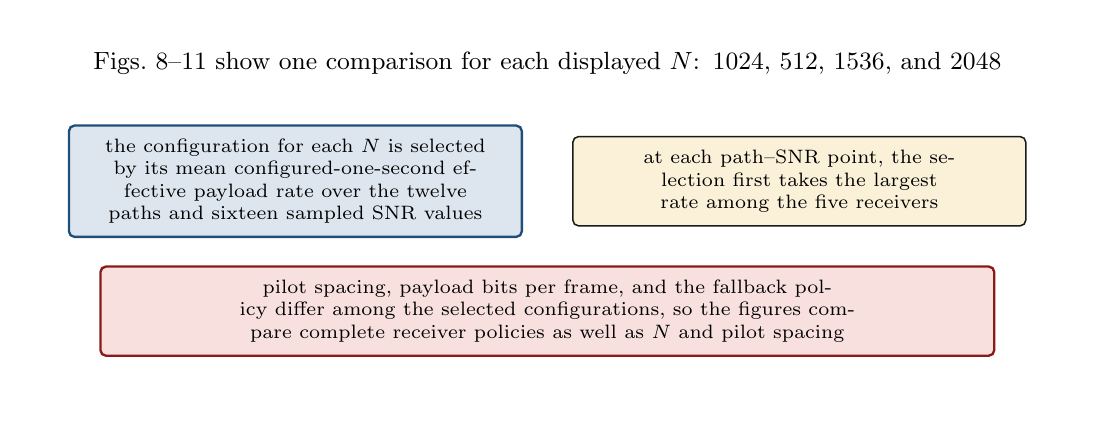
\begin{tikzpicture}[x=1cm,y=1cm]
    \path[use as bounding box] (-6.6,-2.9) rectangle (6.6,2.0);
    \node[font=\small,text width=11.6cm,align=center] at (0,1.55)
      {Figs.~8--11 show one comparison for each displayed \(N\):
       1024, 512, 1536, and 2048};
    \node[bluecard,text width=5.4cm,font=\scriptsize] at (-3.2,0.05)
      {the configuration for each \(N\) is selected by its mean
       configured-one-second effective payload rate over the twelve paths
       and sixteen sampled SNR values};
    \node[card,text width=5.4cm,font=\scriptsize] at (3.2,0.05)
      {at each path--SNR point, the selection first takes the largest
       rate among the five receivers};
    \node[badcard,text width=11.0cm,font=\scriptsize] at (0,-1.60)
      {pilot spacing, payload bits per frame, and the fallback policy
       differ among the selected configurations, so the figures compare
       complete receiver policies as well as \(N\) and pilot spacing};
  \end{tikzpicture}
  \bottomnote{Fig.~8 uses \(N=1024\), CP~64, code rate \(\tfrac14\),
    outer/inner pilot spacing 8/8, and a configured pilot percentage of
    25.000\%.  The other three figures state their own selected
    configurations the same way.}
\end{frame}

% ---------------------------------------------------------------------
\begin{frame}[plain]
  \centering
  \begin{tikzpicture}
    \node[anchor=south west,inner sep=0] (img) at (0,0)
      {\includegraphics[width=0.98\paperwidth,height=0.86\textheight,
        keepaspectratio]{red_ber_receivers}};
    \begin{scope}[x={(img.south east)},y={(img.north west)}]
      \only<2->{
      \node[draw=accentred,fill=paper,fill opacity=0.93,text opacity=1,line width=0.6pt,rounded corners=1.5pt,align=center,inner sep=2.5pt,font=\tiny,text width=3.3cm] (c8a) at (0.44,0.665) {hollow markers: zero observed errors; the floor is 0.5 divided by the payload bits tested, not a measured BER};
      \draw[redarr] (c8a.north west) -- (0.28,0.752);
      \node[draw=accentred,fill=paper,fill opacity=0.93,text opacity=1,line width=0.6pt,rounded corners=1.5pt,align=center,inner sep=2.5pt,font=\tiny,text width=3.3cm] (c8b) at (0.44,0.885) {on RED1/H1 both \(C,z\) policies reach the floor while the baselines flatten far above it};
      \draw[redarr] (c8b.west) -- (0.31,0.878);
      \node[draw=accentred,fill=paper,fill opacity=0.93,text opacity=1,line width=0.6pt,rounded corners=1.5pt,align=center,inner sep=2.5pt,font=\tiny,text width=3.3cm] (c8c) at (0.115,0.62) {the panel legend records exact curve coincidences: here OFDM$+$LDPC $=$ JUNA-Direct-\(C,z\), the fallback whenever the CRC gate fails};
      \draw[redarr] (c8c.north) -- (0.155,0.775);
      \node[draw=accentred,fill=paper,fill opacity=0.93,text opacity=1,line width=0.6pt,rounded corners=1.5pt,align=center,inner sep=2.5pt,font=\tiny,text width=8.8cm] (c8d) at (0.5,0.028) {the curves that carry the JUNA-\(C,z\) output use moving averages of \(\log_{10}\) bit error rate with two points on each side; the others use one; points with no observed bit error are not averaged, and markers show the averaged values};
      }
    \end{scope}
  \end{tikzpicture}\par
  {\tiny\color{inkgray}Fig.~8, $N=1024$ of \texttt{juna\_joint\_ieee.tex}\par}
\end{frame}
% ---------------------------------------------------------------------
\begin{frame}[plain]
  \centering
  \begin{tikzpicture}
    \node[anchor=south west,inner sep=0] (img) at (0,0)
      {\includegraphics[width=0.98\paperwidth,height=0.86\textheight,
        keepaspectratio]{red_ber_receivers_n512}};
    \begin{scope}[x={(img.south east)},y={(img.north west)}]
      \only<2->{
      \node[draw=accentred,fill=paper,fill opacity=0.93,text opacity=1,line width=0.6pt,rounded corners=1.5pt,align=center,inner sep=2.5pt,font=\tiny,text width=8.2cm] (cn) at (0.5,0.035) {\(N=512\), spacing 5/5, configured pilot percentage 40.000\%.  Here a JUNA-\(C,z\) candidate that fails the 16-bit CRC is replaced by the receiver's own Partial-FFT output; JUNA-Direct-\(C,z\) falls back to OFDM$+$LDPC.};
      }
    \end{scope}
  \end{tikzpicture}\par
  {\tiny\color{inkgray}Fig.~9, $N=512$ of \texttt{juna\_joint\_ieee.tex}\par}
\end{frame}
% ---------------------------------------------------------------------
\begin{frame}[plain]
  \centering
  \begin{tikzpicture}
    \node[anchor=south west,inner sep=0] (img) at (0,0)
      {\includegraphics[width=0.98\paperwidth,height=0.86\textheight,
        keepaspectratio]{red_ber_receivers_n1536}};
    \begin{scope}[x={(img.south east)},y={(img.north west)}]
      \only<2->{
      \node[draw=accentred,fill=paper,fill opacity=0.93,text opacity=1,line width=0.6pt,rounded corners=1.5pt,align=center,inner sep=2.5pt,font=\tiny,text width=8.2cm] (cn) at (0.5,0.035) {\(N=1536\), spacing 5/7, configured pilot percentage 34.286\%.  The fallback policies match the \(N=512\) comparison, so the four figures compare complete receiver policies as well as \(N\) and pilot spacing.};
      }
    \end{scope}
  \end{tikzpicture}\par
  {\tiny\color{inkgray}Fig.~10, $N=1536$ of \texttt{juna\_joint\_ieee.tex}\par}
\end{frame}
% ---------------------------------------------------------------------
\begin{frame}[plain]
  \centering
  \begin{tikzpicture}
    \node[anchor=south west,inner sep=0] (img) at (0,0)
      {\includegraphics[width=0.98\paperwidth,height=0.86\textheight,
        keepaspectratio]{red_ber_receivers_n2048}};
    \begin{scope}[x={(img.south east)},y={(img.north west)}]
      \only<2->{
      \node[draw=accentred,fill=paper,fill opacity=0.93,text opacity=1,line width=0.6pt,rounded corners=1.5pt,align=center,inner sep=2.5pt,font=\tiny,text width=8.2cm] (cn) at (0.5,0.035) {\(N=2048\), spacing 5/10, configured pilot percentage 30.000\%.  The same reading applies: hollow markers are the measurement floor, and the legends record exact curve coincidences.};
      }
    \end{scope}
  \end{tikzpicture}\par
  {\tiny\color{inkgray}Fig.~11, $N=2048$ of \texttt{juna\_joint\_ieee.tex}\par}
\end{frame}

% =====================================================================
% 2. The quantity on the vertical axis
% =====================================================================
\begin{frame}{The quantity on the vertical axis}
  \centering
  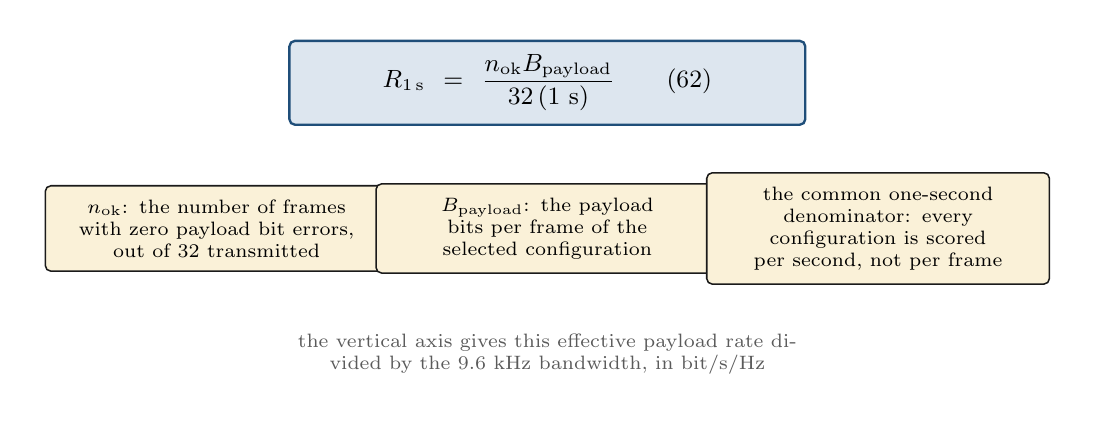
\begin{tikzpicture}[x=1cm,y=1cm]
    \path[use as bounding box] (-6.6,-2.9) rectangle (6.6,2.0);
    \node[bluecard,text width=6.2cm] at (0,1.30)
      {$\displaystyle R_{\mathrm{1\,s}}=
        \frac{n_{\mathrm{ok}}B_{\mathrm{payload}}}{32\,(1~\mathrm{s})}
        \qquad\text{(62)}$};
    \node[card,text width=4.0cm,font=\scriptsize] (a) at (-4.2,-0.55)
      {$n_{\mathrm{ok}}$: the number of frames\\with zero payload bit
       errors,\\out of 32 transmitted};
    \node[card,text width=4.0cm,font=\scriptsize] (b) at (0,-0.55)
      {$B_{\mathrm{payload}}$: the payload\\bits per frame of the\\
       selected configuration};
    \node[card,text width=4.0cm,font=\scriptsize] (c) at (4.2,-0.55)
      {the common one-second\\denominator: every\\configuration is scored\\
       per second, not per frame};
    \node[font=\scriptsize,color=inkgray,text width=11.5cm,align=center]
      at (0,-2.15)
      {the vertical axis gives this effective payload rate divided by the
       9.6~kHz bandwidth, in bit/s/Hz};
  \end{tikzpicture}
  \bottomnote{A frame counts only when every payload bit is exact.  Hence
    the curve rewards configurations that both carry many bits and decode
    them without error.}
\end{frame}

% =====================================================================
% 4. One panel
% =====================================================================
\begin{frame}{One panel}
  \centering
  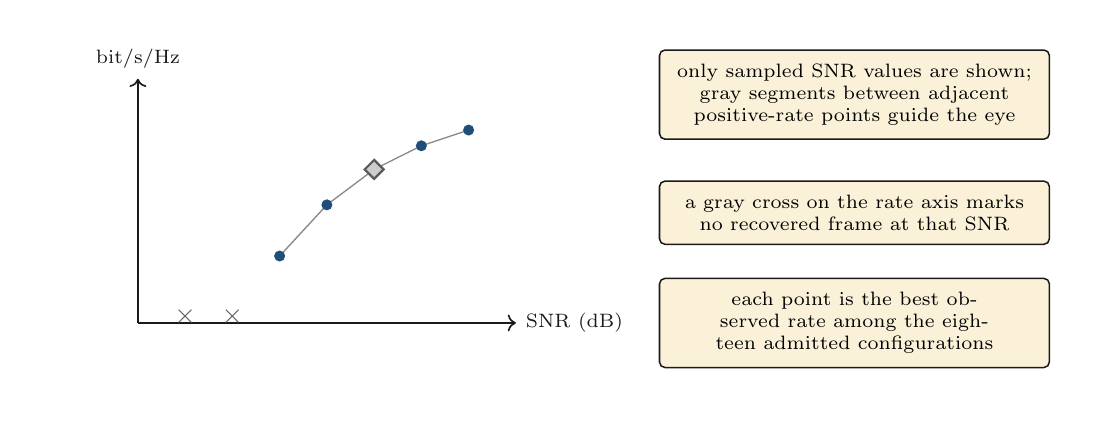
\begin{tikzpicture}[x=1cm,y=1cm]
    \path[use as bounding box] (-6.6,-2.9) rectangle (6.6,2.0);
    \begin{scope}[shift={(-2.9,-0.35)}]
      \draw[->,line width=0.6pt,color=ink] (-2.3,-1.4) -- (2.5,-1.4)
        node[right,font=\scriptsize] {SNR (dB)};
      \draw[->,line width=0.6pt,color=ink] (-2.3,-1.4) -- (-2.3,1.7)
        node[above,font=\scriptsize] {bit/s/Hz};
      % no recovered frame: gray cross on the rate axis
      \node[font=\normalsize,color=inkgray] at (-1.7,-1.32) {$\times$};
      \node[font=\normalsize,color=inkgray] at (-1.1,-1.32) {$\times$};
      % positive-rate points joined by gray guide segments
      \draw[line width=0.5pt,color=inkgray!70]
        (-0.5,-0.55) -- (0.1,0.10) -- (0.7,0.55) -- (1.3,0.85)
        -- (1.9,1.05);
      \fill[accentblue] (-0.5,-0.55) circle (0.07);
      \fill[accentblue] (0.1,0.10) circle (0.07);
      \draw[line width=0.8pt,color=inkgray,fill=inkgray!30,rotate around={45:(0.7,0.55)}]
        (0.7-0.085,0.55-0.085) rectangle (0.7+0.085,0.55+0.085);
      \fill[accentblue] (1.3,0.85) circle (0.07);
      \fill[accentblue] (1.9,1.05) circle (0.07);
    \end{scope}
    \node[card,text width=4.6cm,font=\scriptsize] at (3.9,1.15)
      {only sampled SNR values are shown; gray segments between adjacent
       positive-rate points guide the eye};
    \node[card,text width=4.6cm,font=\scriptsize] at (3.9,-0.35)
      {a gray cross on the rate axis marks no recovered frame at that SNR};
    \node[card,text width=4.6cm,font=\scriptsize] at (3.9,-1.75)
      {each point is the best observed rate among the eighteen admitted
       configurations};
  \end{tikzpicture}
  \bottomnote{The panel here is schematic; the printed figure carries the
    data.  Every point answers one question: at this path and SNR, what is
    the largest zero-error payload rate any admitted configuration and
    receiver achieved?}
\end{frame}

% =====================================================================
% 5. Point color and the receiver letters
% =====================================================================
\begin{frame}{Point color and the receiver letters}
  \centering
  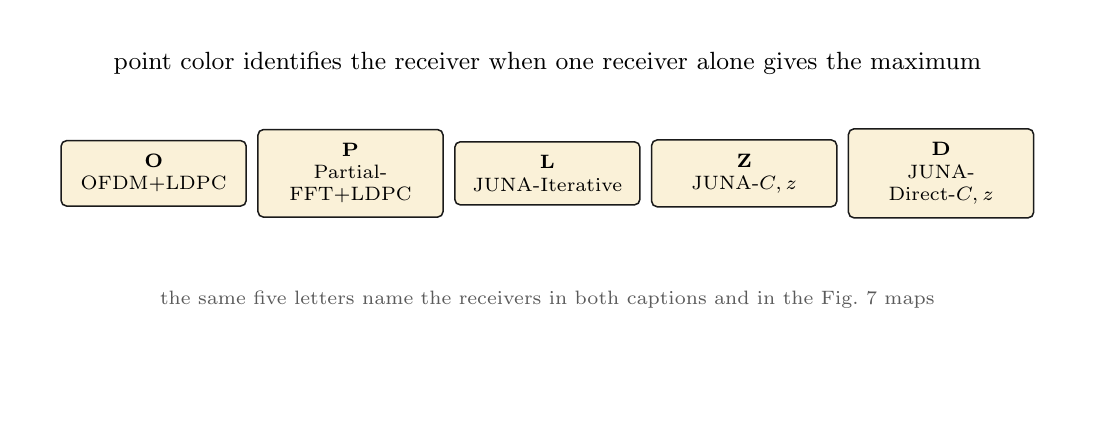
\begin{tikzpicture}[x=1cm,y=1cm]
    \path[use as bounding box] (-6.6,-2.9) rectangle (6.6,2.0);
    \node[font=\small,text width=11.6cm,align=center] at (0,1.55)
      {point color identifies the receiver when one receiver alone gives
       the maximum};
    \node[card,text width=2.0cm,font=\scriptsize] at (-5.0,0.15)
      {\textbf{O}\\OFDM$+$LDPC};
    \node[card,text width=2.0cm,font=\scriptsize] at (-2.5,0.15)
      {\textbf{P}\\Partial-FFT$+$LDPC};
    \node[card,text width=2.0cm,font=\scriptsize] at (0,0.15)
      {\textbf{L}\\JUNA-Iterative};
    \node[card,text width=2.0cm,font=\scriptsize] at (2.5,0.15)
      {\textbf{Z}\\JUNA-\(C,z\)};
    \node[card,text width=2.0cm,font=\scriptsize] at (5.0,0.15)
      {\textbf{D}\\JUNA-Direct-\(C,z\)};
    \node[font=\scriptsize,color=inkgray,text width=10.6cm,align=center]
      at (0,-1.45)
      {the same five letters name the receivers in both captions and in
       the Fig.~7 maps};
  \end{tikzpicture}
  \bottomnote{When no single receiver wins, the point turns gray and its
    shape says who tied --- the next slide.}
\end{frame}

% =====================================================================
% 6. The tie markers
% =====================================================================
\begin{frame}{The tie markers}
  \centering
  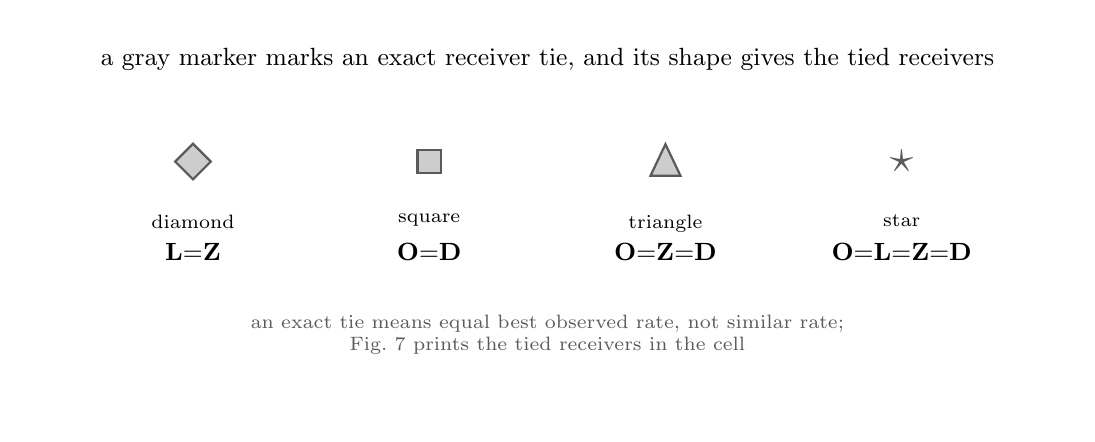
\begin{tikzpicture}[x=1cm,y=1cm]
    \path[use as bounding box] (-6.6,-2.9) rectangle (6.6,2.0);
    \node[font=\small] at (0,1.60)
      {a gray marker marks an exact receiver tie, and its shape gives the
       tied receivers};
    % diamond
    \draw[line width=0.8pt,color=inkgray,fill=inkgray!30,rotate around={45:(-4.5,0.3)}]
      (-4.5-0.16,0.3-0.16) rectangle (-4.5+0.16,0.3+0.16);
    \node[font=\scriptsize,anchor=north] at (-4.5,-0.25) {diamond};
    \node[font=\small\bfseries,anchor=north] at (-4.5,-0.62) {L$=$Z};
    % square
    \draw[line width=0.8pt,color=inkgray,fill=inkgray!30]
      (-1.5-0.15,0.3-0.15) rectangle (-1.5+0.15,0.3+0.15);
    \node[font=\scriptsize,anchor=north] at (-1.5,-0.25) {square};
    \node[font=\small\bfseries,anchor=north] at (-1.5,-0.62) {O$=$D};
    % triangle
    \draw[line width=0.8pt,color=inkgray,fill=inkgray!30]
      (1.5,0.52) -- (1.5-0.19,0.12) -- (1.5+0.19,0.12) -- cycle;
    \node[font=\scriptsize,anchor=north] at (1.5,-0.25) {triangle};
    \node[font=\small\bfseries,anchor=north] at (1.5,-0.62) {O$=$Z$=$D};
    % star
    \node[font=\LARGE,color=inkgray] at (4.5,0.30) {$\star$};
    \node[font=\scriptsize,anchor=north] at (4.5,-0.25) {star};
    \node[font=\small\bfseries,anchor=north] at (4.5,-0.62) {O$=$L$=$Z$=$D};
    \node[font=\scriptsize,color=inkgray,text width=10.8cm,align=center]
      at (0,-1.90)
      {an exact tie means equal best observed rate, not similar rate;\\
       Fig.~7 prints the tied receivers in the cell};
  \end{tikzpicture}
  \bottomnote{A tie is common where the frame decodes cleanly for several
    receivers at once; the tie says the receivers agree, not that the
    comparison failed.}
\end{frame}

% =====================================================================
% 7. The ribbon
% =====================================================================
\begin{frame}{The ribbon}
  \centering
  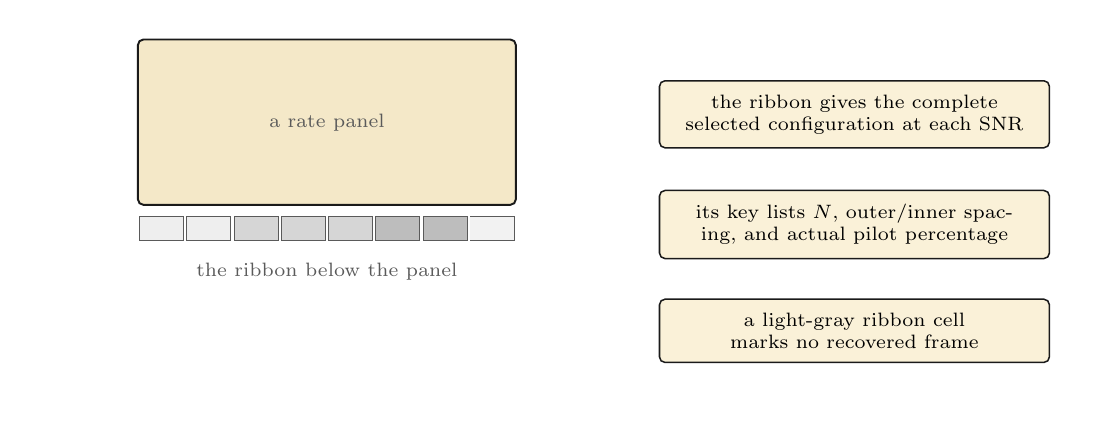
\begin{tikzpicture}[x=1cm,y=1cm]
    \path[use as bounding box] (-6.6,-2.9) rectangle (6.6,2.0);
    \begin{scope}[shift={(-2.9,0.35)}]
      \draw[panelbox] (-2.3,-0.6) rectangle (2.5,1.5);
      \node[font=\scriptsize,color=inkgray] at (0.1,0.45) {a rate panel};
      \foreach \x/\sh in {-2.0/10, -1.4/10, -0.8/25, -0.2/25, 0.4/25,
                          1.0/40, 1.6/40, 2.2/40}{
        \fill[inkgray!\sh] (\x-0.28,-1.05) rectangle (\x+0.28,-0.75);
        \draw[line width=0.3pt,color=inkgray] (\x-0.28,-1.05)
          rectangle (\x+0.28,-0.75);
      }
      \fill[inkgray!8] (2.2-0.28,-1.05) rectangle (2.2+0.28,-0.75);
      \node[font=\scriptsize,color=inkgray,anchor=north] at (0.1,-1.22)
        {the ribbon below the panel};
    \end{scope}
    \node[card,text width=4.6cm,font=\scriptsize] at (3.9,0.90)
      {the ribbon gives the complete selected configuration at each SNR};
    \node[card,text width=4.6cm,font=\scriptsize] at (3.9,-0.50)
      {its key lists \(N\), outer/inner spacing, and actual pilot
       percentage};
    \node[card,text width=4.6cm,font=\scriptsize] at (3.9,-1.85)
      {a light-gray ribbon cell marks no recovered frame};
  \end{tikzpicture}
  \bottomnote{The ribbon is where configuration changes show: when the best
    point switches from one \(N\) or pilot spacing to another, the ribbon
    cell changes with it.}
\end{frame}

% ---------------------------------------------------------------------
\begin{frame}[plain]
  \centering
  \begin{tikzpicture}
    \node[anchor=south west,inner sep=0] (img) at (0,0)
      {\includegraphics[width=0.98\paperwidth,height=0.86\textheight,
        keepaspectratio]{red_effective_payload_rate_explorer}};
    \begin{scope}[x={(img.south east)},y={(img.north west)}]
      \only<2->{
      \node[draw=accentred,fill=paper,fill opacity=0.93,text opacity=1,line width=0.6pt,rounded corners=1.5pt,align=center,inner sep=2.5pt,font=\tiny,text width=3.4cm] (c6a) at (0.4,0.315) {RED4/H1 at 10~dB: admitting JUNA-Direct-\(C,z\) raises the maximum to 1763.125~bit/s and flips the selected 1024 spacing from 8/8 to 5/10};
      \draw[redarr] (c6a.west) -- (0.175,0.322);
      \node[draw=accentred,fill=paper,fill opacity=0.93,text opacity=1,line width=0.6pt,rounded corners=1.5pt,align=center,inner sep=2.5pt,font=\tiny,text width=3.0cm] (c6b) at (0.4,0.5) {RED3/H1 at 8~dB: the other Direct point, 181.5 to 226.875~bit/s};
      \draw[redarr] (c6b.west) -- (0.163,0.45);
      \node[draw=accentred,fill=paper,fill opacity=0.93,text opacity=1,line width=0.6pt,rounded corners=1.5pt,align=center,inner sep=2.5pt,font=\tiny,text width=2.6cm] (c6c) at (0.115,0.6) {crosses: no recovered frame --- 40 of the 192 points};
      \draw[redarr] (c6c.south) -- (0.117,0.43);
      \node[draw=accentred,fill=paper,fill opacity=0.93,text opacity=1,line width=0.6pt,rounded corners=1.5pt,align=center,inner sep=2.5pt,font=\tiny,text width=8.6cm] (c6d) at (0.5,0.035) {JUNA-\(C,z\) is in the maximum at 138 of the 152 positive points --- alone at 73 (orange), tied with JUNA-Iterative at 51 (gray diamonds); Partial-FFT$+$LDPC is not a maximum at any point};
      }
    \end{scope}
  \end{tikzpicture}\par
  {\tiny\color{inkgray}Fig.~6 of \texttt{juna\_joint\_ieee.tex}\par}
\end{frame}
% =====================================================================
% 8. Figure 7: the two maps
% =====================================================================
\begin{frame}{Figure 7: the two maps}
  \centering
  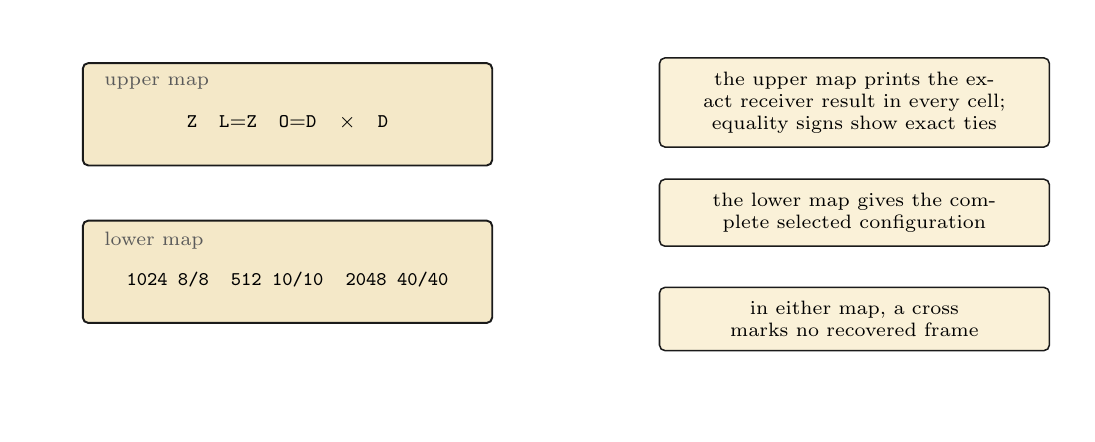
\begin{tikzpicture}[x=1cm,y=1cm]
    \path[use as bounding box] (-6.6,-2.9) rectangle (6.6,2.0);
    \begin{scope}[shift={(-3.3,0.0)}]
      \draw[panelbox] (-2.6,0.25) rectangle (2.6,1.55);
      \node[font=\scriptsize,color=inkgray,anchor=west] at (-2.45,1.30)
        {upper map};
      \node[font=\scriptsize] at (0,0.80)
        {\texttt{Z}\quad\texttt{L$=$Z}\quad\texttt{O$=$D}\quad
         \texttt{$\times$}\quad\texttt{D}};
      \draw[panelbox] (-2.6,-1.75) rectangle (2.6,-0.45);
      \node[font=\scriptsize,color=inkgray,anchor=west] at (-2.45,-0.70)
        {lower map};
      \node[font=\scriptsize] at (0,-1.20)
        {\texttt{1024 8/8}\quad\texttt{512 10/10}\quad
         \texttt{2048 40/40}};
    \end{scope}
    \node[card,text width=4.6cm,font=\scriptsize] at (3.9,1.05)
      {the upper map prints the exact receiver result in every cell;
       equality signs show exact ties};
    \node[card,text width=4.6cm,font=\scriptsize] at (3.9,-0.35)
      {the lower map gives the complete selected configuration};
    \node[card,text width=4.6cm,font=\scriptsize] at (3.9,-1.70)
      {in either map, a cross marks no recovered frame};
  \end{tikzpicture}
  \bottomnote{The reading loop: find a point in Fig.~6, then read the same
    path and SNR cell in Fig.~7 --- the upper map names the receivers, the
    lower map names the configuration.  The maps here are schematic; the
    printed figure carries the data.}
\end{frame}

% ---------------------------------------------------------------------
\begin{frame}[plain]
  \centering
  \begin{tikzpicture}
    \node[anchor=south west,inner sep=0] (img) at (0,0)
      {\includegraphics[width=0.98\paperwidth,height=0.86\textheight,
        keepaspectratio]{red_effective_payload_selection_explorer}};
    \begin{scope}[x={(img.south east)},y={(img.north west)}]
      \only<2->{
      \node[draw=accentred,fill=paper,fill opacity=0.93,text opacity=1,line width=0.6pt,rounded corners=1.5pt,align=center,inner sep=2.5pt,font=\tiny,text width=3.2cm] (c7a) at (0.82,0.94) {the one point where JUNA-Iterative alone gives the maximum: RED1/H1 at 18~dB};
      \draw[redarr] (c7a.west) -- (0.612,0.868);
      \node[draw=accentred,fill=paper,fill opacity=0.93,text opacity=1,line width=0.6pt,rounded corners=1.5pt,align=center,inner sep=2.5pt,font=\tiny,text width=3.2cm] (c7b) at (0.62,0.585) {the two Direct cells: RED3/H1 at 8~dB and RED4/H1 at 10~dB --- the same two points as in Fig.~6};
      \draw[redarr] (c7b.north west) -- (0.328,0.722);
      \draw[redarr] (c7b.west) -- (0.383,0.666);
      \node[draw=accentred,fill=paper,fill opacity=0.93,text opacity=1,line width=0.6pt,rounded corners=1.5pt,align=center,inner sep=2.5pt,font=\tiny,text width=3.4cm] (c7c) at (0.62,0.33) {blue cells: \(N=512\) is selected at 10 positive points; \(N=1024\) at 139, \(N=1536\) at 2, \(N=2048\) at 1, \(N=4096\) never};
      \draw[redarr] (c7c.west) -- (0.34,0.40);
      }
    \end{scope}
  \end{tikzpicture}\par
  {\tiny\color{inkgray}Fig.~7 of \texttt{juna\_joint\_ieee.tex}\par}
\end{frame}
% =====================================================================
% 9. Takeaway
% =====================================================================
\begin{frame}[plain]
  \centering
  \vspace{0.8cm}
  {\bfseries\LARGE Reading the Red result figures\par}
  \vspace{0.45cm}
    {\large the twelve panels are three hydrophones of one array observed
   in four segments of one deployment~~(Fig.~5)\par}
  \vspace{0.30cm}
  {\large the payload bit error rate figures show the same twelve paths
   at one selected configuration per \(N\)\par}
  \vspace{0.30cm}
  {\large every point: the best observed zero-error payload rate at one
   path and SNR~~(62)\par}
  \vspace{0.30cm}
  {\large color names the sole winner; gray shapes name exact ties\par}
  \vspace{0.30cm}
  {\large the ribbon and the lower map name the selected configuration\par}
  \vspace{0.30cm}
  {\large the upper map prints every receiver result, ties included\par}

  \vspace{0.45cm}
  {\itshape receiver and configuration should be compared together: no one
   choice gives every observed maximum\par}
\end{frame}

\end{document}
